\subsubsection{Numerical Analysis of Quantum Chernoff Bounds}
Below is a numerical implimentation for the validation of the Helstrom Bounds over the limit of N.

\begin{lstlisting}[style=pythonstyle, caption={Includes}]
import numpy as np
import matplotlib.pyplot as plt
from scipy.optimize import minimize_scalar
from qutip import rand_dm, ket2dm, tensor
\end{lstlisting}


Defining the two random density matrices 
$$
\hat{\rho}_0 = \begin{pmatrix}
0.5276 & -0.4914 + 0.0466i \\
-0.4914 - 0.0466i & 0.4724
\end{pmatrix}
$$
$$
\hat{\rho}_1 = \begin{pmatrix}
0.4214 & 0.1045 + 0.2534i \\
0.1045 - 0.2534i & 0.5786
\end{pmatrix}
$$
\begin{lstlisting}[style=pythonstyle, caption={Defining the two state with random density matrix}]
rho0 = rand_dm(2, seed=809)
rho1 = rand_dm(2, seed=593)
print(rho0)
print(rho1)
\end{lstlisting}


\begin{lstlisting}[style=pythonstyle, caption={Defining a function to calculate the matrix power of rho}]
def mat_power(rho, t):
    vals, vecs = rho.eigenstates()
    vals = np.maximum(vals, 0)
    return sum(v**t * ket2dm(vec) for v, vec in zip(vals, vecs))
\end{lstlisting}

\begin{lstlisting}[style=pythonstyle, caption={Defining a function to return the Qs}]
def Qs(r0, r1, s):
    return np.real((mat_power(r0, s) * mat_power(r1, 1-s)).tr())
\end{lstlisting}

\begin{lstlisting}[style=pythonstyle, caption={Gaussian state discrimination with QuTiP: Helstrom bound and Quantum Chernoff bound}]
# Minimize Qs wrt s within the bounds 0 < s < 1
res = minimize_scalar(lambda s: Qs(rho0, rho1, s), bounds=(0.01,0.99), method='bounded')
\end{lstlisting}


\begin{lstlisting}[style=pythonstyle, caption={Extracting the results}]
# Extract the results
Q = res.fun
s_opt = res.x
Q_half = Qs(rho0, rho1, 0.5)
xi = -np.log(Q)
print(f"s*={s_opt:.4f}  Q={Q:.6f}  Q_half={Q_half:.6f}  xi={xi:.6f}")
\end{lstlisting}


\begin{lstlisting}[style=pythonstyle, caption={Defining a function to return the N trails accumulated helstrom bounds}]
def helstrom_N(r0, r1, N):
    r0N   = tensor([r0]*N)
    r1N   = tensor([r1]*N)
    Gamma = r1N - r0N
    evals = Gamma.eigenenergies()
    del r0N, r1N, Gamma
    return 0.5*(1.0 - 0.5*np.sum(np.abs(evals)))
\end{lstlisting}


\begin{lstlisting}[style=pythonstyle, caption={Computing the helstrom bounds}]
N_max  = 10
N_vals = np.arange(1, N_max+1)
print("Computing Helstrom...")
PE_exact = np.array([helstrom_N(rho0, rho1, N) for N in N_vals])
print("Done:", PE_exact)
\end{lstlisting}


\begin{lstlisting}[style=pythonstyle, caption={Calculating the probabilities of error}]
PE_QCB   = 0.5 * Q**N_vals
PE_bhat  = 0.5 * Q_half**N_vals
log_exact = np.log(np.maximum(PE_exact,1e-15)) / N_vals
log_QCB   = np.log(PE_QCB)  / N_vals
log_bhat  = np.log(PE_bhat) / N_vals
\end{lstlisting}


\begin{lstlisting}[style=pythonstyle, caption={Finding the probability of error for different thetas over different bounds}]
theta_vals = np.linspace(0,1,40)
pe_h, pe_q, pe_b, pe_f = [],[],[],[]
for th in theta_vals:
    r1t = th*rho1 + (1-th)*rho0
    ev  = (r1t-rho0).eigenenergies()
    pe_h.append(0.5*(1-0.5*np.sum(np.abs(ev))))
    res2 = minimize_scalar(lambda s,r=r1t: Qs(rho0,r,s),bounds=(0.01,0.99),method='bounded')
    pe_q.append(0.5*res2.fun)
    pe_b.append(0.5*Qs(rho0,r1t,0.5))
    r0h = mat_power(rho0,0.5)
    F   = float(np.real(((r0h*r1t*r0h).sqrtm()).tr()))
    pe_f.append((1-np.clip(F,0,1))/2)
\end{lstlisting}



\begin{lstlisting}[style=pythonstyle, caption={Plotting}]
plt.figure(figsize=(10, 7))
s_values = np.linspace(0.01, 0.99, 1000)
Q_values = [Qs(rho0, rho1, s_) for s_ in s_values]
plt.plot(s_values, Q_values)
plt.xlabel('s')
plt.ylabel(R'$Q_s$')
plt.savefig('../figures/Q_vs_s.png', dpi=300)
plt.show()


plt.figure(figsize=(10, 7))
plt.axhline(-xi, label='Assymptotic Limit')
plt.plot(N_vals, log_exact, label='Exact')
plt.plot(N_vals, log_QCB, label='Quantum Chernoff bound')
plt.plot(N_vals, log_bhat, label='Bhattacharyya bound')
plt.xlabel('N')
plt.ylabel(R'$\frac{ln(P_E)}{N}$')
plt.grid()
plt.legend()
plt.savefig('../figures/QCB.png', dpi=300)
plt.show()


plt.figure(figsize=(10, 7))
plt.plot(theta_vals,pe_h,'-',lw=2.5,label='Exact Helstrom')
plt.plot(theta_vals,pe_q,'--',lw=2,  label='Quantum Chernoff bound')
plt.plot(theta_vals,pe_b,':',lw=2,  label='Bhattacharyya bound')
plt.plot(theta_vals,pe_f,'-.',lw=2,  label='Fidelity lower bound')
plt.xlabel(R'$\theta$')
plt.ylabel('Error Probability')
plt.legend()
plt.savefig('../figures/P_E.png', dpi=300)
plt.show()
\end{lstlisting}


\subsubsection{Results}
\begin{figure}[H]
    \centering
    \begin{minipage}{0.45\textwidth}
        \centering
        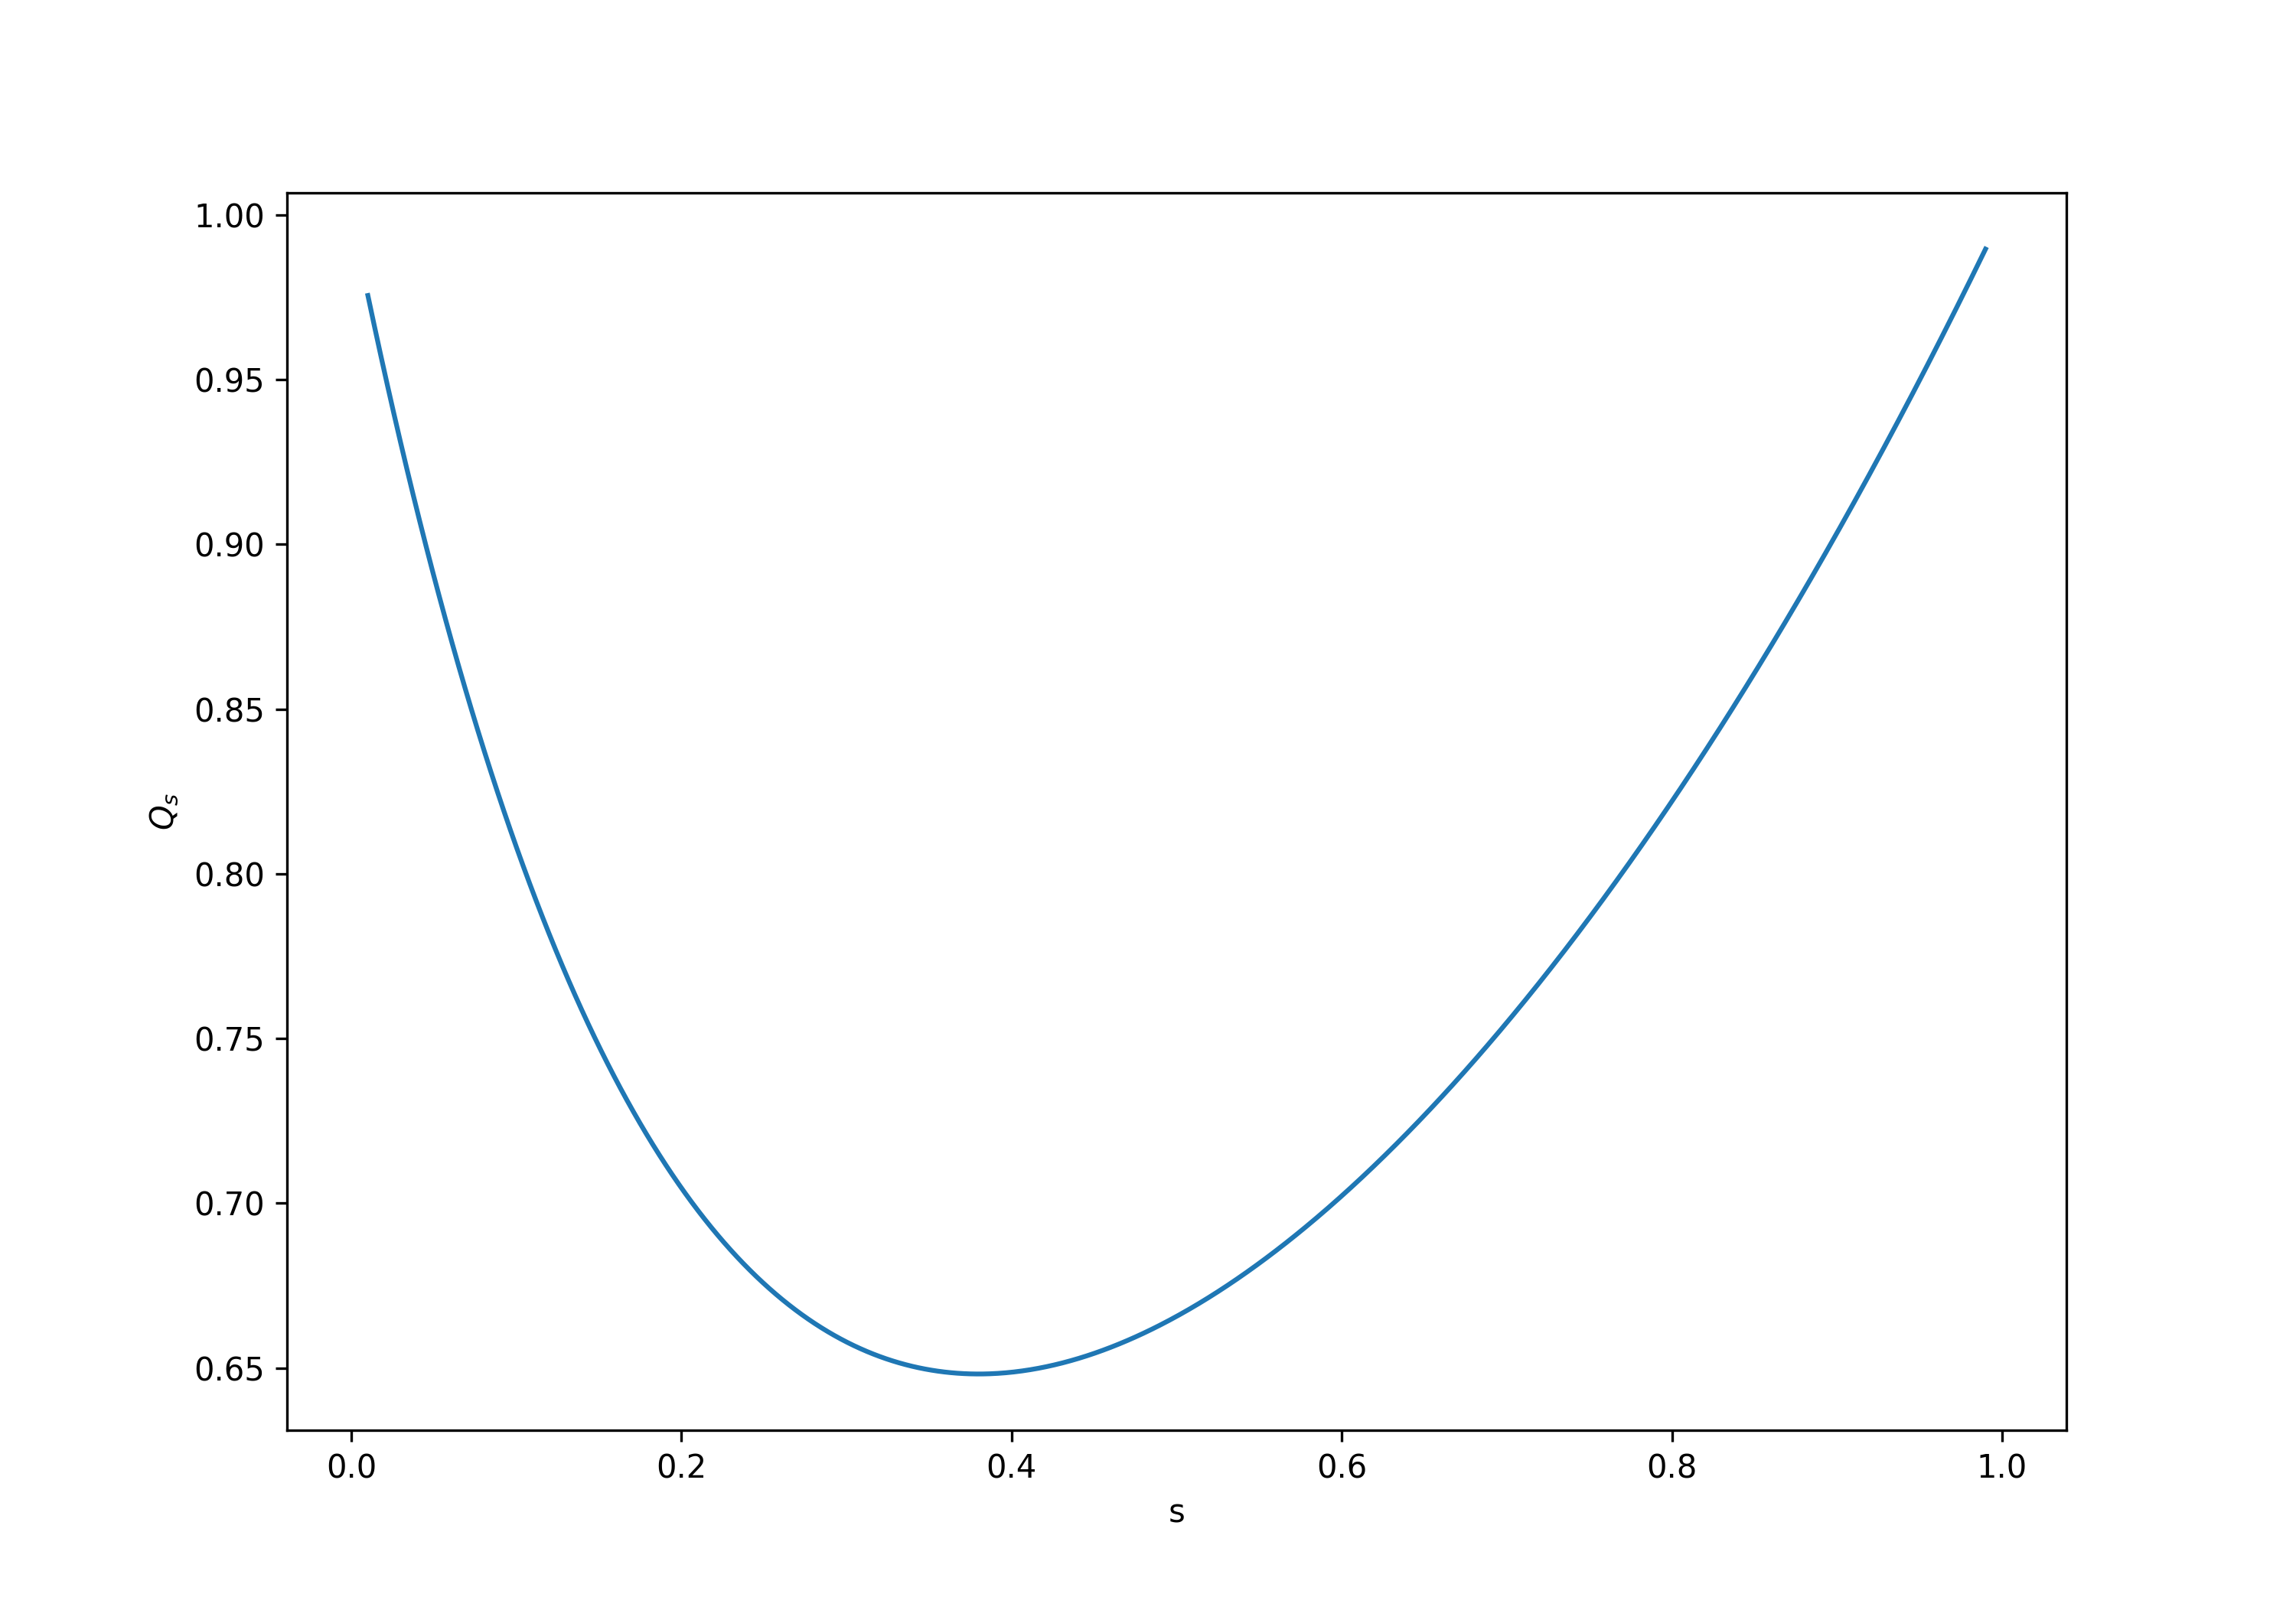
\includegraphics[width=\textwidth]{figures/Q_vs_s.png}
        \caption{Convex nature of Qs}
        \label{fig:31}
    \end{minipage}
    \hfill
    \begin{minipage}{0.45\textwidth}
        \centering
        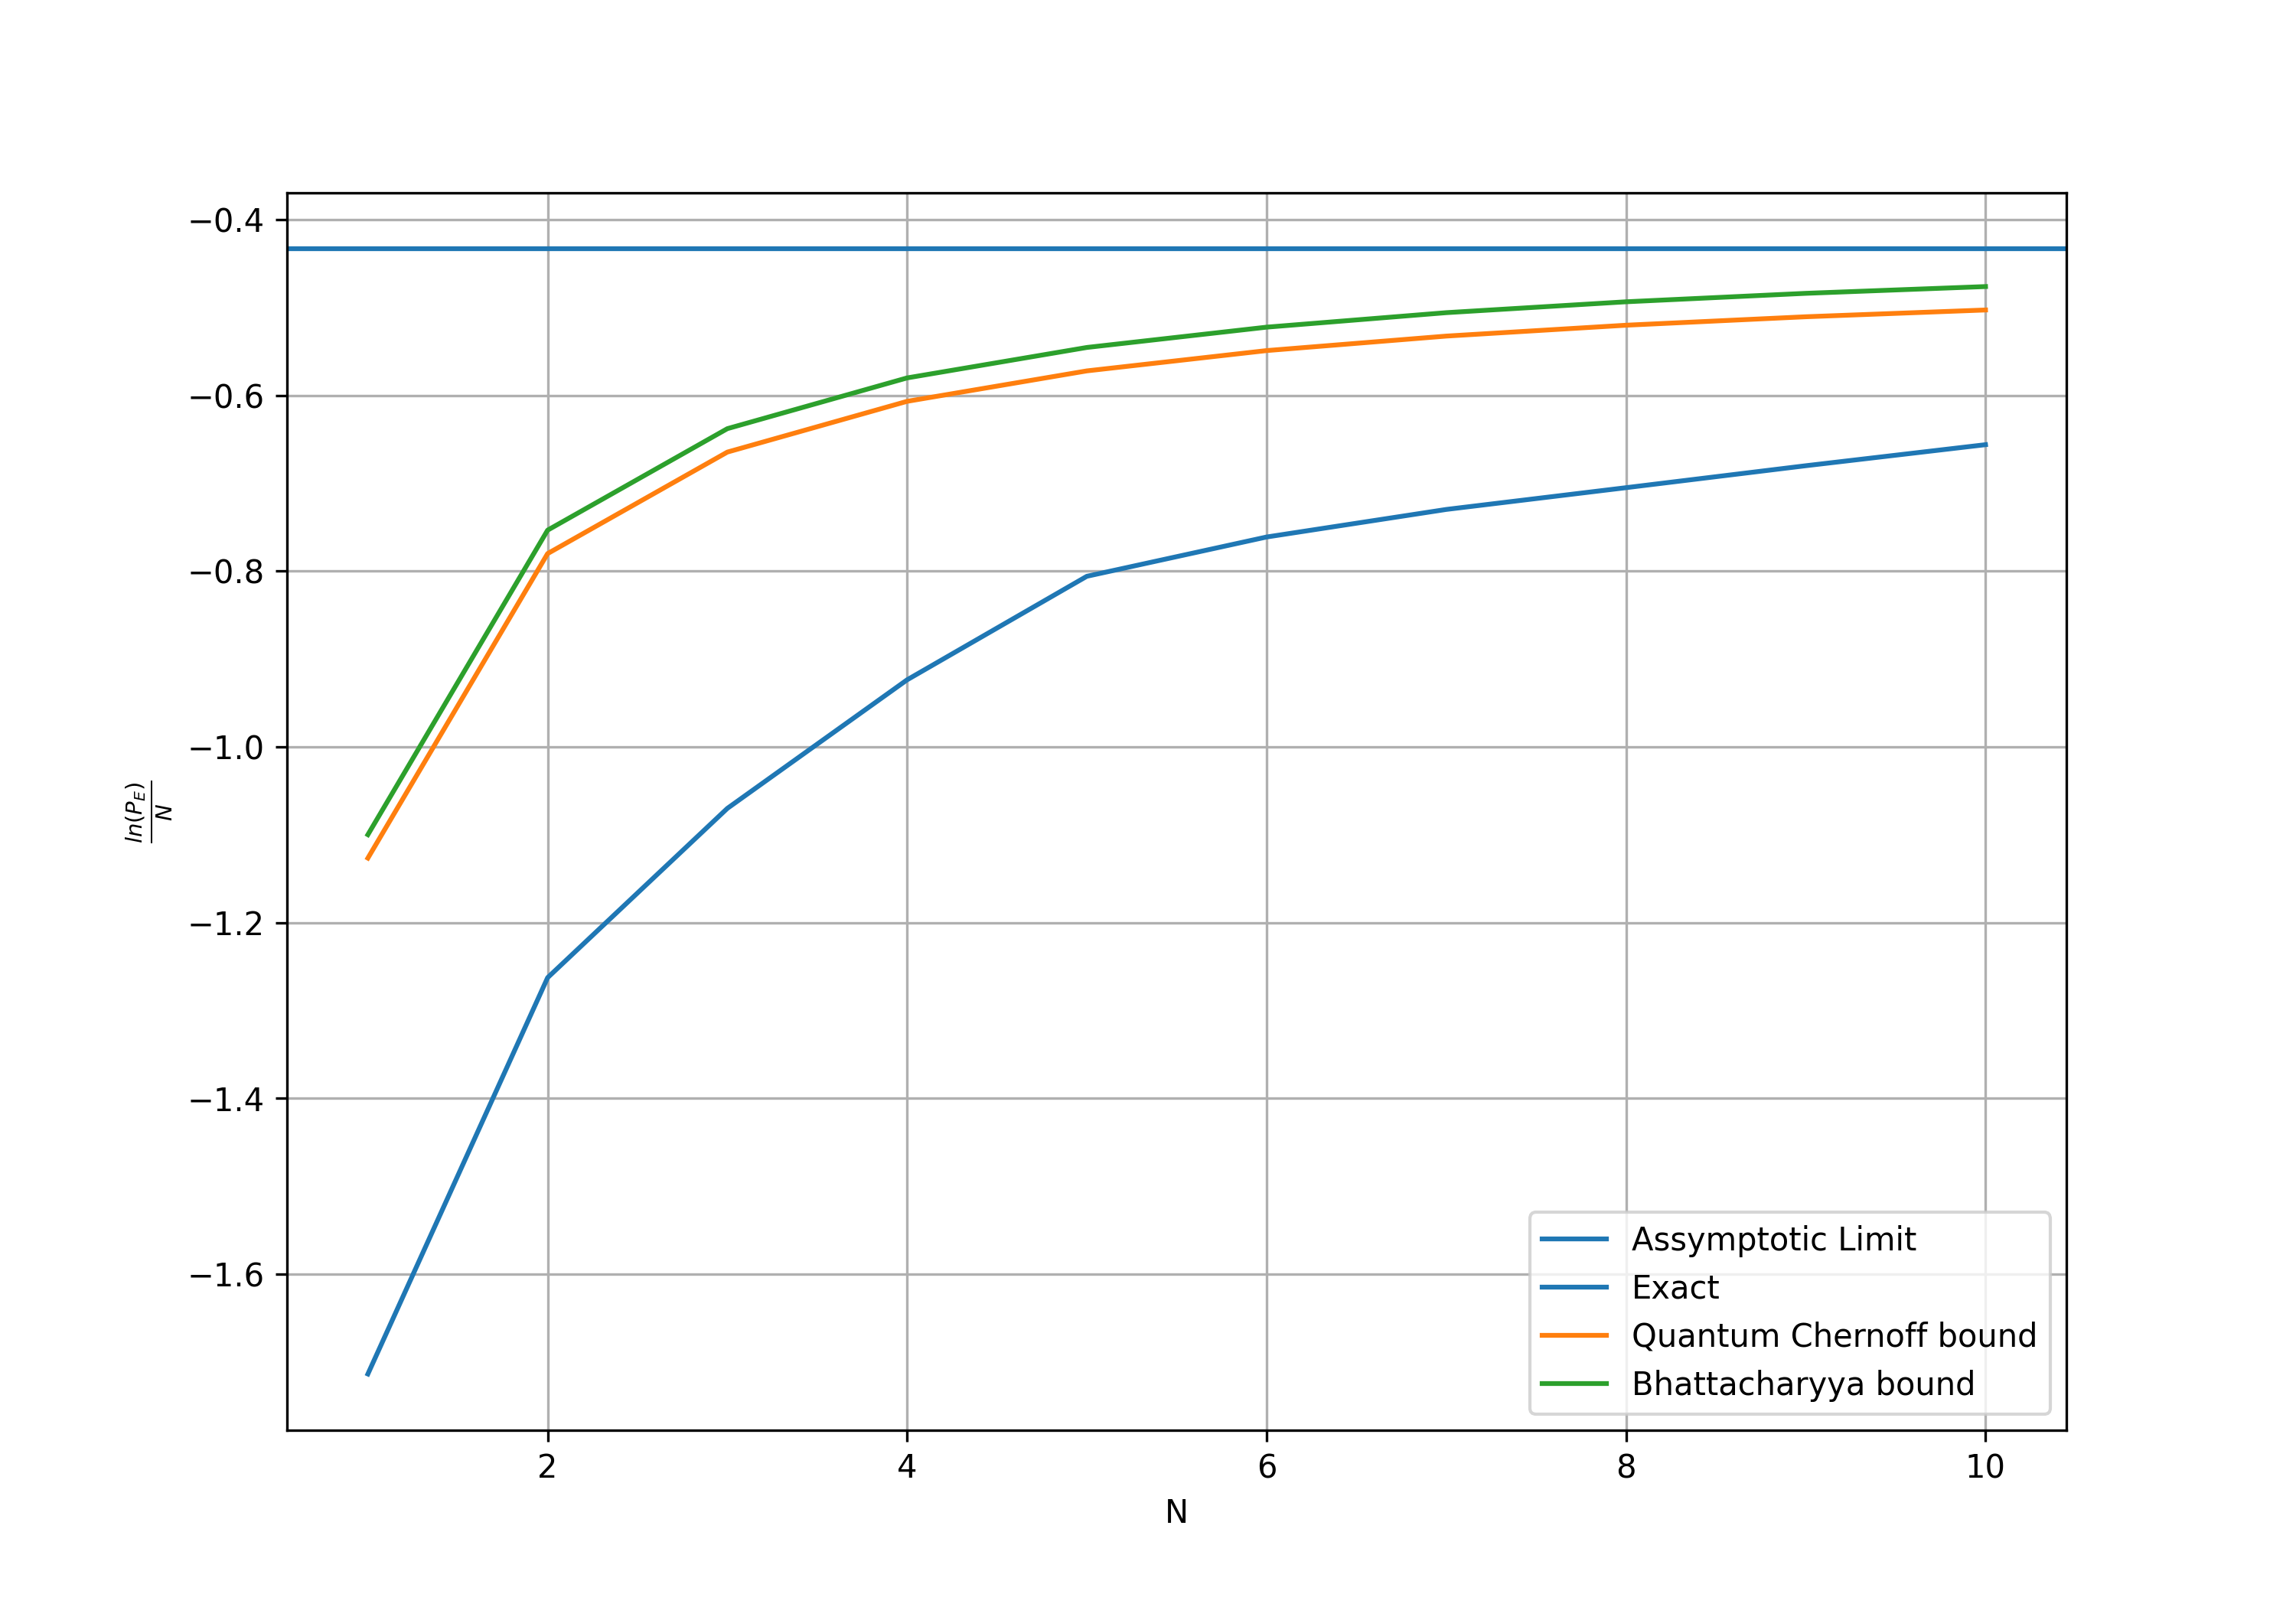
\includegraphics[width=\textwidth]{figures/QCB.png}
        \caption{Different Bounds as N increases}
        \label{fig:32}
    \end{minipage}

    \vspace{0.5cm}
    \begin{minipage}{0.45\textwidth}
        \centering
        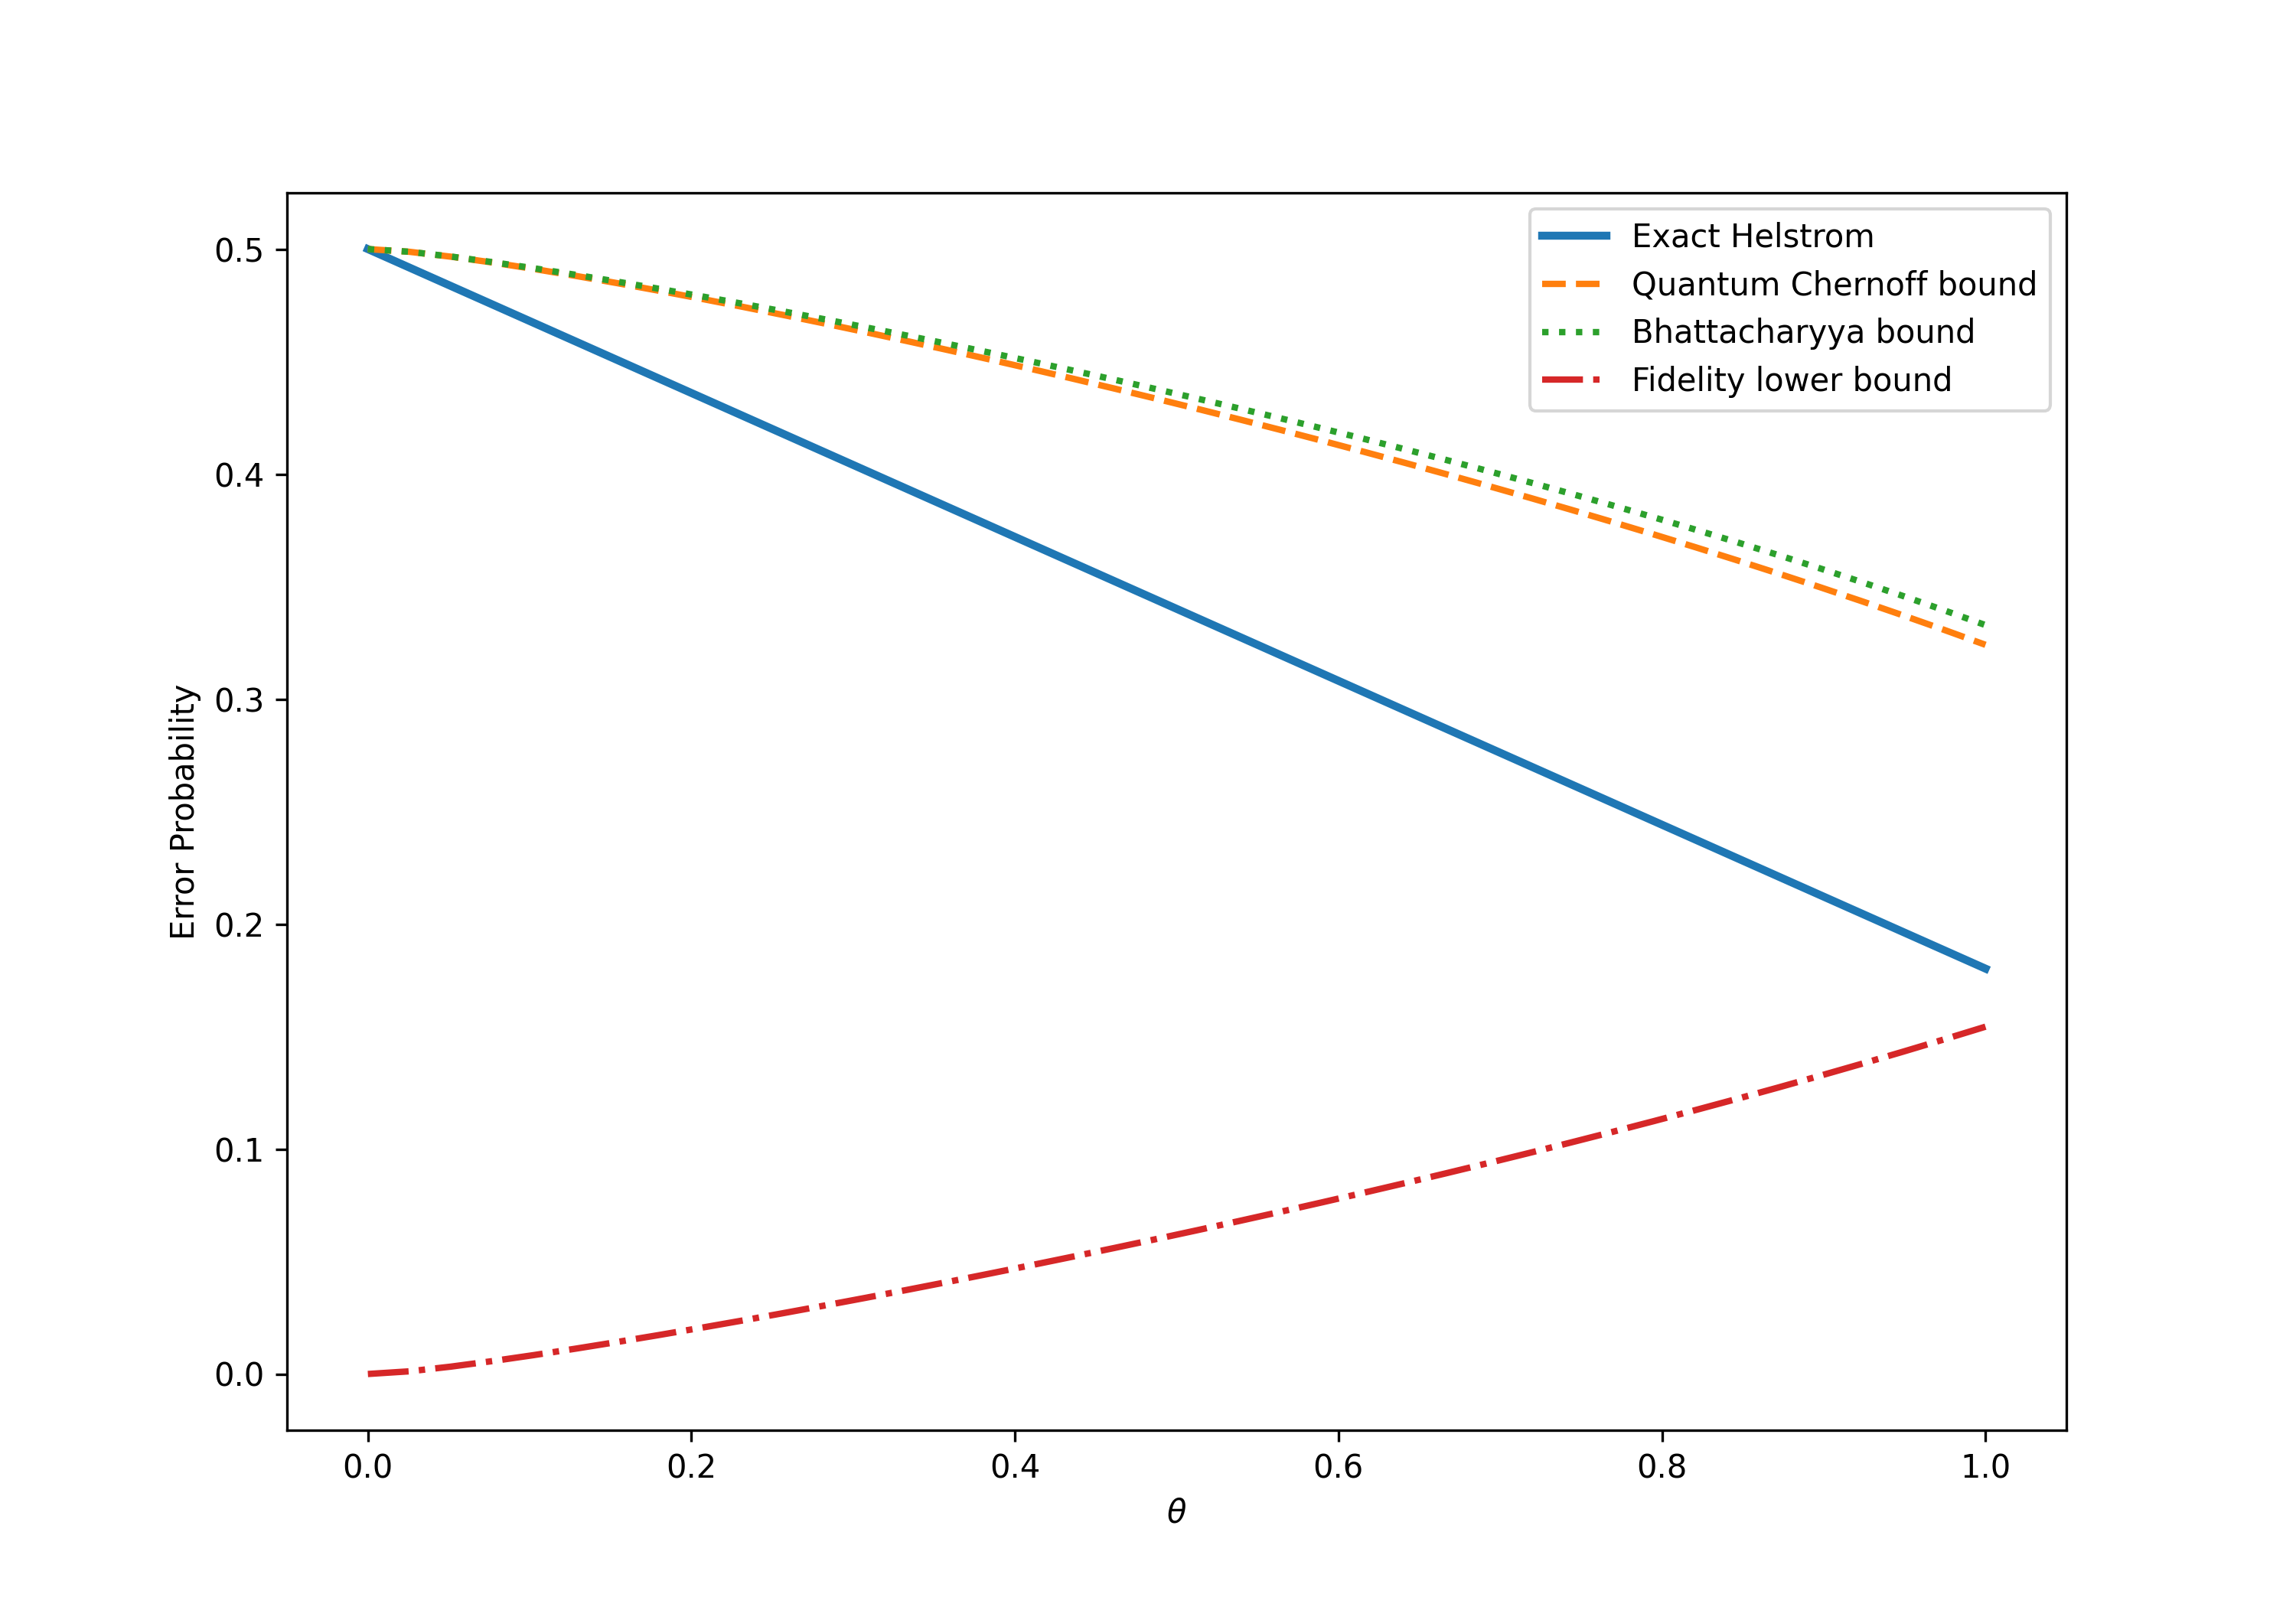
\includegraphics[width=\textwidth]{figures/P_E.png}
        \caption{Error Probability within Bounds}
        \label{fig:33}
    \end{minipage}
\end{figure}
\textbf{Interpretation}
fig~\ref{fig:31} clearly shows the convex nature of $Q_s$ over s for $s \in [0, 1]$, with a unique minima at near $s \approx 0.47$. This visually confirms the theoretical results discussed before. Moreover, as minimum of s is close to $\frac{1}{2}$, we can see in fig~\ref{fig:32}, that the Quantum Chernoff Bounds and the Bhattacharyya bounds are close, but since it is not exactly 0.5, so the Quantum Chernoff Bound converges faster. Moreover, fig~\ref{fig:32} also shows the asymptotic nature limit of the bounds $-\kappa = ln(Q)$ as N becomes large, confirming the exponential decay of the error probability $P_E = e^{-\kappa N}$. Also, the Helstrom Bound lies below the chernoff bounds as predicted by the equation $P_{E, N}^{min} \le \frac{1}{2}Q^N$. In fig~\ref{fig:33}, as $\theta$ varies from 0 to 1, the state $\hat{\rho}_1(\theta) = \theta \hat{\rho}_1 + (1 - \theta) \hat{\rho}_0$, interpolates between the two states. At $\theta = 0$, both hypothesis are identical and is seen in the plot as 0.5, with maximum error. As $\theta$ increases, the states becomes more distinct and the error probability starts decreasing. Moreover, it also follows the ordering eq~\ref{eq:ineq}
